\chapter{Shape Representation}
\label{ch:shape-representation}

% TODO details depth cameras and laser/radar sensors
Coming back to the original problem of this thesis, the goal is to complete
shapes. As we want to learn both the shape prior as well as the proposed
shape completion approaches using 3D convolutional neural networks, we require
grid-based representations of the observations, \ie point clouds from KITTI
\cite{GeigerLenzUrtasun:2012,GeigerLenzStillerUrtasun:2013}, and the shapes, \ie
meshes from ShapeNet \cite{ChangFunkhouserGuibasSavarese:2015}.
As foreshadowed in Chapter \ref{ch:problem}, we primarily rely
on occupancy grids for representing the observations and both occupancy
grids and signed distance functions for representing shapes.
In the following we briefly formalize both modalities in detail.

\section{Point Clouds}

Point clouds are unordered sets of 3D points.
%where we ignore the details
%of acquisition for simplicity\footnote{
%  On KITTI, for example, point clouds are acquired using a Velodyne sensor,
%  see Chapter \ref{ch:data} for details, which internally
%  imposes an order of the captured 3D points.
%}.
In our formulation of Problem \ref{problem}, point clouds correspond
to a raw version of the observations $\mathcal{X}$:

% TODO remove mathcal for matrices?
\begin{definition}
  A point cloud $\mathcal{P} = \{p_1, \ldots, p_N\} \subseteq \mathbb{R}^3$ is a
  set of points with dimensions corresponding to width (horizontal),
  height (vertical) and depth in this order.
\end{definition}

% TODO tensor always indices, 3D always coordinates
We note that the dimensions are not coherent with the introduced tensor dimensions,
\ie $H \times W \times D$. While this might seem confusing, we decided to follow
common practice in computer vision and deep learning where the first
dimension of tensors refers to the height of an image or a volume\footnote{
  This is motivated by popular computer vision libraries such as OpenCV
  (\url{http://opencv.org/}) and tools such as SciPy (\url{https://www.scipy.org/})
  as well as deep learning frameworks, \eg Torch (\url{http://torch.ch/}).
}. This means, that height and width axes need to be swapped when 
voxelizing point clouds into occupancy grids, see Section
\ref{sec:shape-representation-occupancy}. Point clouds from KITTI
have already been illustrated in Figure \ref{fig:introduction}.

\begin{figure}
  \centering
  \begin{tikzpicture}
    %\node[rectangle,draw=black,fill=white] at (0,0) {\includegraphics[height=2cm]{data/kitti/snapshot_01_rect}};
    %\node[rectangle,draw=black,fill=white] at (5,0) {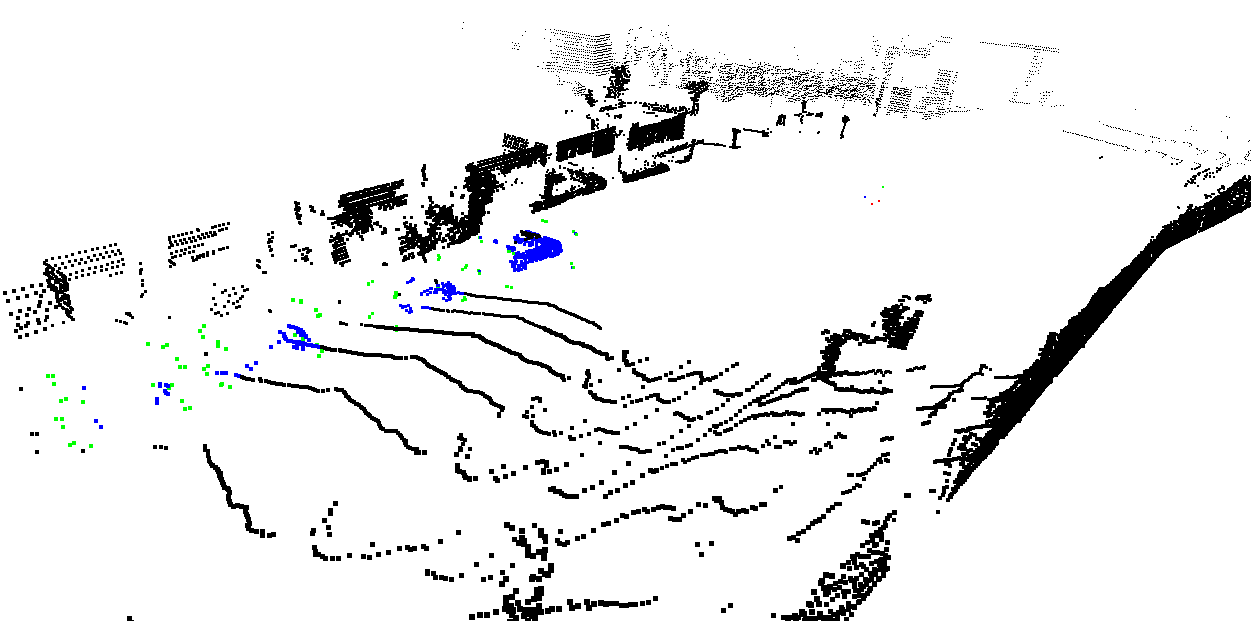
\includegraphics[height=2cm]{data/kitti/snapshot03_rect}};
    
    % https://tex.stackexchange.com/questions/40840/put-a-node-behind-another-in-a-tikz-diagram
    %\begin{scope}[on background layer]
    %  \node[] at (3,-1.5) {\includegraphics[width=5.5cm,trim={4cm 1cm 13cm 3cm},clip]{data/kitti/snapshot_00_rect_fade}};
    %\end{scope}
    
    %\node[rectangle,draw=black] at (-0.9,-2.75) {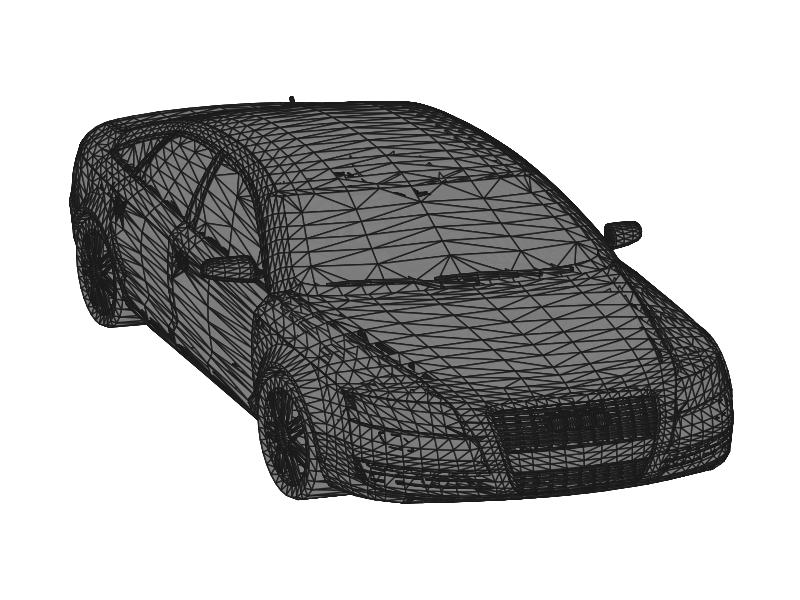
\includegraphics[height=2cm]{data/shapenet/simplification/1104f0924e03f2b6fc5886e868449015}};
    %\node[rectangle,draw=black] at (2.6,-2.75) {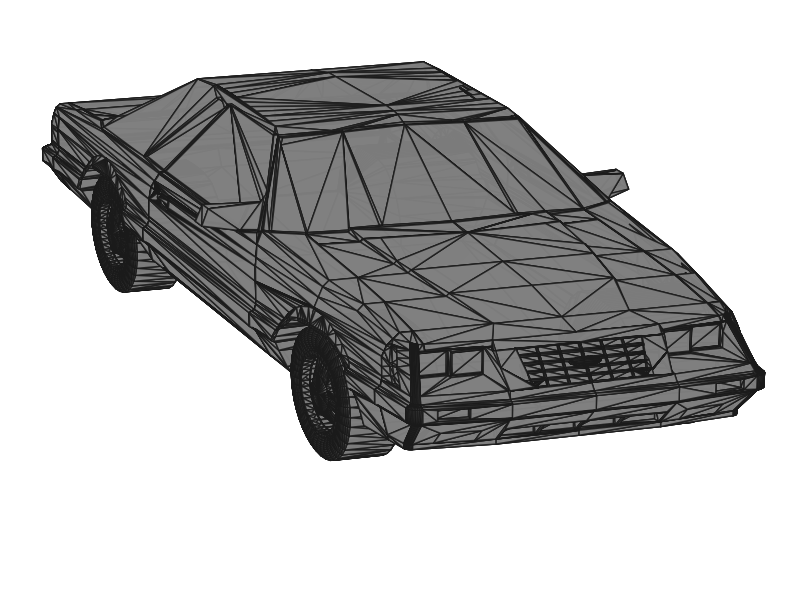
\includegraphics[height=2cm]{data/shapenet/simplification/1089cbe82dc0e72133d7c9e122eec9b6}};
    
    \node at (0, 1.5) {Mesh};
    \node[rectangle,draw=black,fill=white] (m) at (0,0) {
      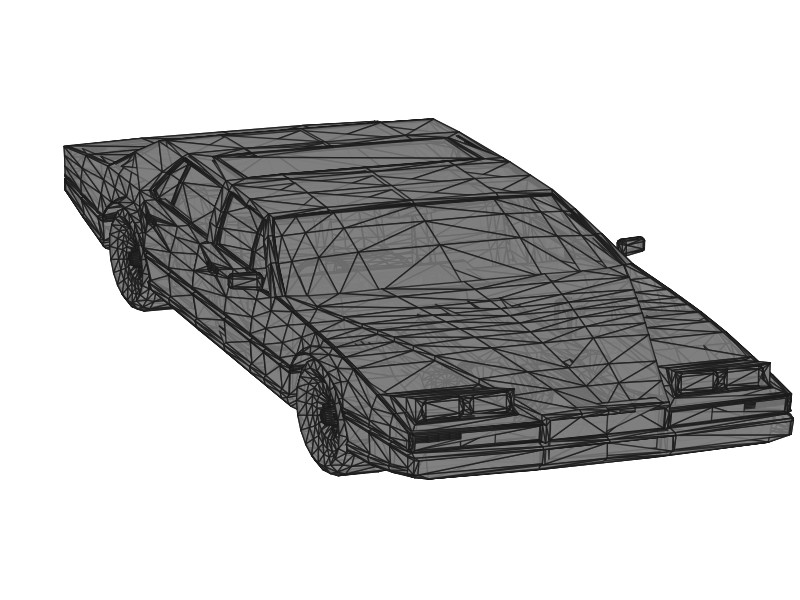
\includegraphics[height=2.25cm]{data/shapenet/dd84236f0ef27765a134736201a79843}
    };
    
    \node at (6, 1.5) {Simplified Mesh};
    \node[rectangle,draw=black,fill=white] (s) at (6,0) {
      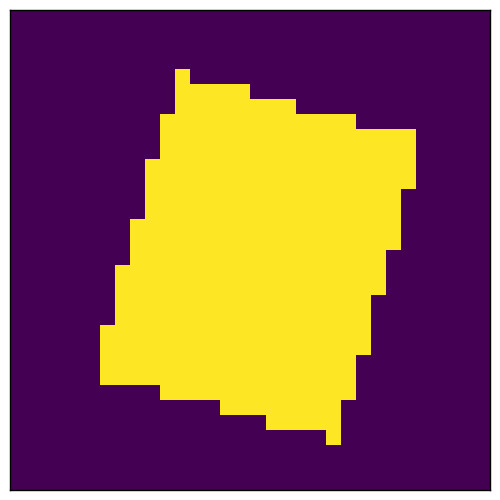
\includegraphics[height=2.25cm,trim={1cm 1cm 1cm 1cm},clip]{data/shapenet/0}
    };
    
    \node at (12, 1.5) {Occupancy Grid};
    \node[rectangle,draw=black,fill=white] (o) at (12,0) {
      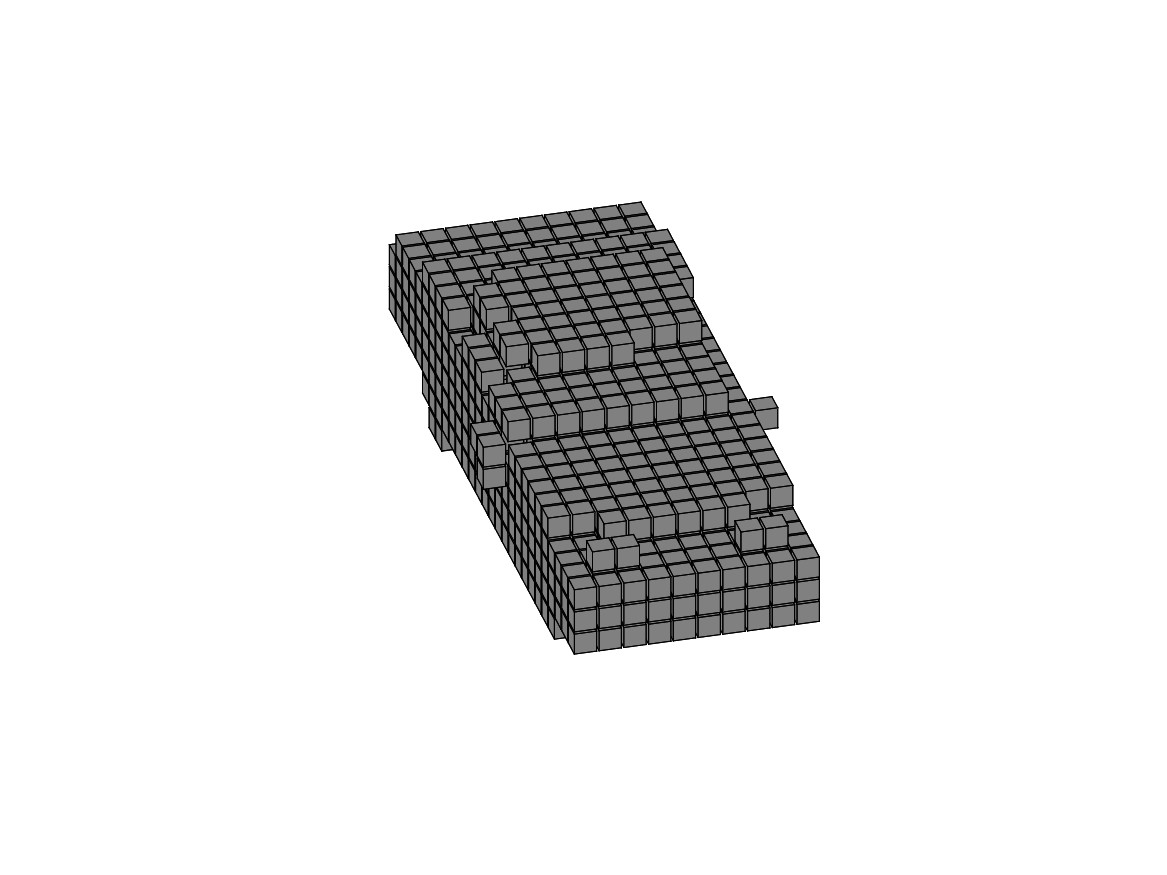
\includegraphics[height=2.25cm,trim={3cm 2cm 3cm 2cm},clip]{data/shapenet/1_output_75}
    };
    
    \node at (3, 0.4) {\small Simplification};
    \node at (9, 0.4) {\small Voxelization};
    \draw[->] (m) -- (s);
    \draw[->] (s) -- (o);
    
    \node at (3.05, -3.75) {Signed Distance Function};
    \node[rectangle,draw=black,fill=white] (sdf) at (3.05,-2.5) {
      \begin{tabular}{@{}c@{}}
        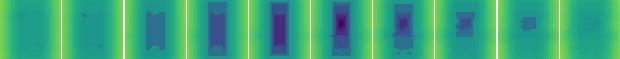
\includegraphics[width=8.4cm]{data/shapenet/1_sdf_output_slices}\\[-6px]
        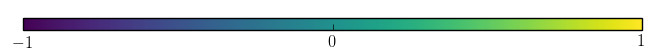
\includegraphics[width=9.05cm]{data/shapenet/sdf_colorbar}
      \end{tabular}
    };
    
    \node at (10, -3) {Distance Transform};
    \draw[-,dashed] (o) -- (12, -2.5);
    \draw[->,dashed] (12,-2.5) -- (sdf);
  \end{tikzpicture}
  \vskip 6px
  
  % TODO short caption
  \caption{Illustration of the used modalities, \ie occupancy grids and
  signed distance functions. In particular, a given triangular mesh is first
  simplified in order to reduce its complexity and obtain a watertight mesh
  which is required for voxelization, \ie to obtain an occupancy grid.
  In this thesis, we derive the corresponding signed distance function from the occupancy
  grid using a distance transform -- as illustrated by the dashed line. We note,
  however, that signed distance functions should in general be derived from
  the original mesh in order to obtain sub-voxel accuracy.}
  \label{fig:shape-representation}
\end{figure}

\section{Meshes}

Another source of information for our problem are datasets
of Computer-Aided Design (CAD) models. In this thesis, we assume that
CAD models are provided as triangular meshes -- we refer to
\cite{BotschKobbelt:2010} for a detailed introduction.
Regarding Problem \ref{problem},
these correspond to a raw version of the shape set $\mathcal{Y}$:

% TODO computation graph mathcal
% TODO wording and \mathcal{M} everywhere
\begin{definition}
  A triangular mesh $\mathcal{M} = (V, F)$ is defined by a set of 
  vertices $V \subseteq \mathbb{R}^3$ and a set of triangular faces
  $F \subseteq \{1,\ldots,|V|\}^3$ such that $f = (f_1, f_2, f_3) \in F$
  defines a triangular face enclosed by the corresponding vertices
  $v_{f_1}$, $v_{f_2}$ and $v_{f_3}$. Faces implicitly also define the edges
  $E(F)$ between the vertices.
\end{definition}

An illustration of a triangular mesh from ShapeNet can be found in Figure
\ref{fig:shape-representation}. The concepts of adjacency and incidency
are naturally extended to triangular meshes. We note that a triangular mesh
only defines the surface of an object. Without additional constraints it is
generally hard to reason about the interior and exterior of the surface
-- and whether the surface is closed.
As we also see in Chapter \ref{ch:data}, this question naturally leads to the
concept of watertight meshes. In the literature \cite[Section~1.3]{BotschKobbelt:2010},
watertight meshes are usually defined as 2-manifold meshes without boundary edges,
see Appendix \ref{ch:appendix-shape-representation} for details.
Another problem, illustrated in Figure \ref{fig:shape-representation}, concerns
very detailed meshes, \ie meshes consisting of a
large number of faces and vertices, often going into the tenth of thousands. 
Therefore, mesh simplification \cite[Chapter~6]{BotschKobbelt:2010} is an important
problem in computer graphics. In Chapter \ref{ch:data} we will present a very
practical approach to compute very rough, simplified meshes. In our case, this algorithm
solves both problems -- obtaining watertight and simplified meshes.

\section{Occupancy Grids}
\label{sec:shape-representation-occupancy}

Given point clouds or watertight meshes, occupancy grids are a natural representation
for applying deep learning techniques. In particular, 3D convolutional neural networks
are able to operate directly on the provided topology and thereby
utilize spatial information. Operating
directly on triangular meshes or point clouds, in contrast, is less straight-forward
regarding a proper representation (\eg for encoding the faces) which would need
to be invariant to the order of faces or points \cite{GarciaGarciaLopez:2016,FanSuGuibas:2016}
and allow to leverage local information
\cite{QiYiSuGuibas:2017,GuoChen:2015,BoscainiVandergheynst:2015,BrunaLeCun:2013}.
Occupancy grids assume a voxelization of the space and
determine, for each voxel, its occupancy. Specifically, a voxel is
considered occupied if it lies inside the interior of the shape or intersects with
its surface. For point clouds, a voxel is considered occupied if it contains at
least one point.

\begin{definition}
  An occupancy grid is a tensor $x \in \{0,1\}^{H \times W \times D}$ where
  the elements $x_i$ are called voxels and $x_i = 1$ corresponds to an occupied
  voxel and $x_i = 0$ determines an unoccupied voxel.
\end{definition}

Occupancy grids can be interpreted as explicit shape representation. With
$H$, $W$ and $D$ being large enough, \ie using high resolution, even small details
of shapes can be captured, \eg see \cite{TatarchenkoBrox:2017}. In Figure
\ref{fig:shape-representation}, we illustrate the voxelization of the shown
simplified mesh.

\section{Signed Distance Functions}
\label{sec:shape-representation-sdf}

In contrast to occupancy grids, signed distance functions are used to define shapes
implicitly.
%Even in the computer graphics literature, where meshes are
%considered parametric representations, signed distance functions are described as
%implicit representation.
In the general case, a signed distance function
can be defined as follows \cite[Chapter~1]{BotschKobbelt:2010}:

% TODO wording and F
\begin{definition}
  Let $F:\mathbb{R}^3 \mapsto \mathbb{R}$ be a continuous function. Then,
  the surface of a shape is implicitly defined by the zero level-set
  $S := \{x \in \mathbb{R}^3 | F(x) = 0\}$ of $F$. As convention, $F$ is negative
  in the interior of the shape and positive in the exterior of the shape.
\end{definition}

%We consider continuous functions only, as we do not want shapes with holes.
The implicit representation through distance functions simplifies the problem
of determining the interior and exterior of a shape. The name stems from the
fact that $F$ is usually taken to be the signed distance to the nearest point
on the surface, \eg
\begin{align}
  |F(x)| = \min_{x_S \in S} \|x - x_S\|_2.
\end{align}
In order to numerically work with signed distance functions, they are usually
defined on a regular grid:

% TODO wording
\begin{definition}
  A signed distance function is a tensor $x \in \mathbb{R}^{H \times W \times D}$
  such that $x_i$ is the signed distance of the center of the corresponding voxel
  to the surface of the shape. It is negative inside the shape, and positive
  outside of it.
\end{definition}

% TODO cite marching cubes
In practice, and as simplification, we are computing signed distance functions
from occupancy grids. This is an important distinction; by using the
occupancy grid representation, we lose accuracy depending
on the used resolution. To re-gain higher accuracy, we could instead utilize a
signed distance function obtained from the original surface
\cite{LorensenCline:1987,BotschKobbelt:2010}; we leave this for future work.

\begin{remark}
  \label{rem:shape-representation-distance-function}
  Given an occupancy grid $x \in \{0,1\}^{H \times W \times D}$, we
  derive the corresponding distance function
  $\text{df}(x) \in \mathbb{R}^{H \times W \times D}$ as
  \begin{align}
    \text{df}_i(x) = \min_{j, x_j = 1} \|i - j\|_2.
  \end{align}
  Similarly, the signed distance function $\text{sdf}(x)$ can be
  defined by combining $\text{df}(x)$ and $\text{df}(1 - x)$
  with the appropriate signs.
\end{remark}

In practice, the conversion from occupancy grids to (signed) distance
functions can be computed using generalized distance transforms
\cite{FelzenswalbHuttenlocher:2012}. To compute the sign,
the interior and exterior must be known; for watertight meshes
the interior and exterior can be determined using occupancy grids
and connected components/flood filling algorithms \cite[Section~3.4]{Szeliski:2011}.
As defined above, we assume the distance function
$\text{df}_i(x)$ to represent the distance to the next occupied voxel $x_j = 1$
such that $\text{df}_i(1 - x)$ is the distance to the next unoccupied voxel.
We also found that using the log signed distance function, \ie
\begin{align}
  \text{lsdf}(x)_i = \sign(\text{sdf}(x)_i) \ln(1 + |\text{sdf}(x)_i|),
\end{align}
aids neural network training -- a strategy also employed for similar representations,
\eg for depth prediction \cite{EigenFergus:2015,EigenFergus:2014,LainaRupprechtNavab:2016}.
Intuitively, the log reduces the range of the prediction problem; in contrast to simple scaling,
however, the range is reduced non-linearly such that the range of small distances (\ie around
the zero level set) is effectively increased at the expense of larger distances.


% TODO remark?
%\begin{remark}
%  Given a signed distance function $\text{sdf}(x) \in \mathbb{R}^{H \times W \times D}$,
%  the log signed distance function is given by
%  \begin{align}
%    \text{lsdf}(x)_i = \sign(\text{sdf}(x)_i) \ln |\text{sdf}(x)_i|.
%  \end{align}
%\end{remark}
